Per "comportamenti automatici" si intende quegli schemi metodologici che vengono generati automaticamente. In questo caso specifico, la parola "comportamento" va a sottolineare la generazione di catene di transazioni, ovvero la creazione di transazioni collegate tra loro mediante il riutilizzo degli output come input (come è stato visto nel capitolo precedente). Con il termine "automatico" si vuole andare a sottolineare un qualcosa che non è "manuale", ovvero non implica l'intervento dell'uomo.

\section{Anonimia delle transazioni}

Come è stato già sottolineato, le transazioni hanno diverse configurazioni a seconda di quanti input e output intervengono nello scambio. Infatti, è largamente probabile che una transazione abbia un solo input, e molteplici output. Oltre a questa struttura, però, la caratteristica più importante di questo sistema è però il completo anonimato delle transazioni. Sebbene all'interno di una transazione possiamo notare gli indirizzi hash tra cui viene effettuato lo scambio, essi non possono essere riconducibili ad un utente reale. Perciò, se si ha una transazione con un input e due output, si noterà uno scambio tra indirizzi bitcoin. 

Per esempio, andando a visualizzare una transazione sul sito \cite{blockchainInfo}, si ottiene quello che si può notare in \textit{figura \ref{fig:realtx}}.
\begin{figure}[htbp]
	\centering
	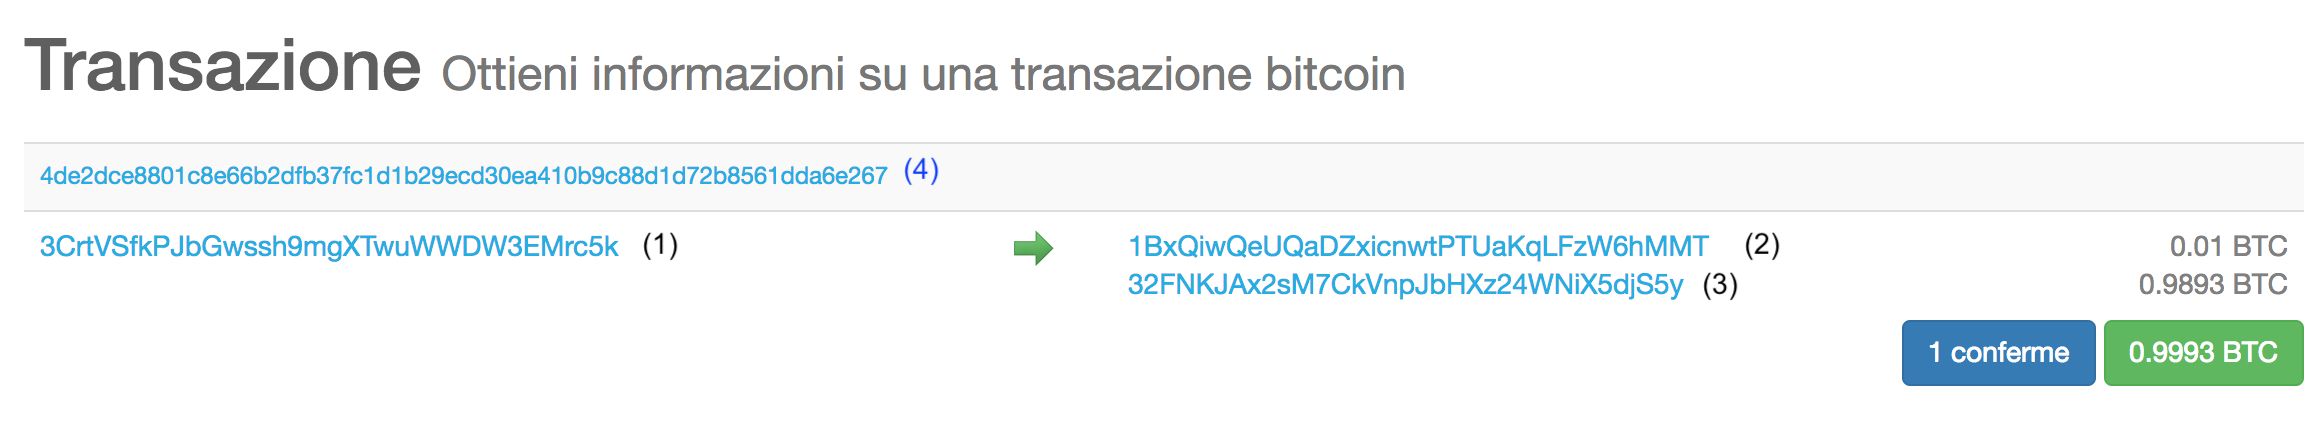
\includegraphics[width = \linewidth]{figure/realtx}
	\caption{\textit{Una transazione del sito Blockchain.info} \cite{blockchainInfo} \label{fig:realtx}}
\end{figure}
Osservando la transazione \textit{(4)}, si osserva che il numero degli output è maggiore del numero degli input. Infatti viene effettuato uno scambio di bitcoin tra l'input \textit{(1)} e gli output \textit{(2) (3)}. Inoltre, al lato della figura sono presenti due bottoni: uno blu, che indica il numero delle conferme che ha ottenuto la transazione, ed uno verde, che indica l'importo bitcoin che viene scambiato. Sopra al bottone verde, gli importi bitcoin ripartiti per i vari indirizzi.

Come ci si aspettava, la transazione identifica degli scambi esclusivamente tra indirizzi bitcoin, rappresentati tramite codici hash. Per andare più a fondo, cliccando su tali codici, si cerca di trovare qualche informazione in più riguardo gli agenti che intervengono nella transazione. Il risultato ottenuto è la \textit{figura \ref{fig:realtxdetails}}
\newline

\begin{figure}[htbp]
	\centering
	\begin{subfigure}[b]{0.8\textwidth}
		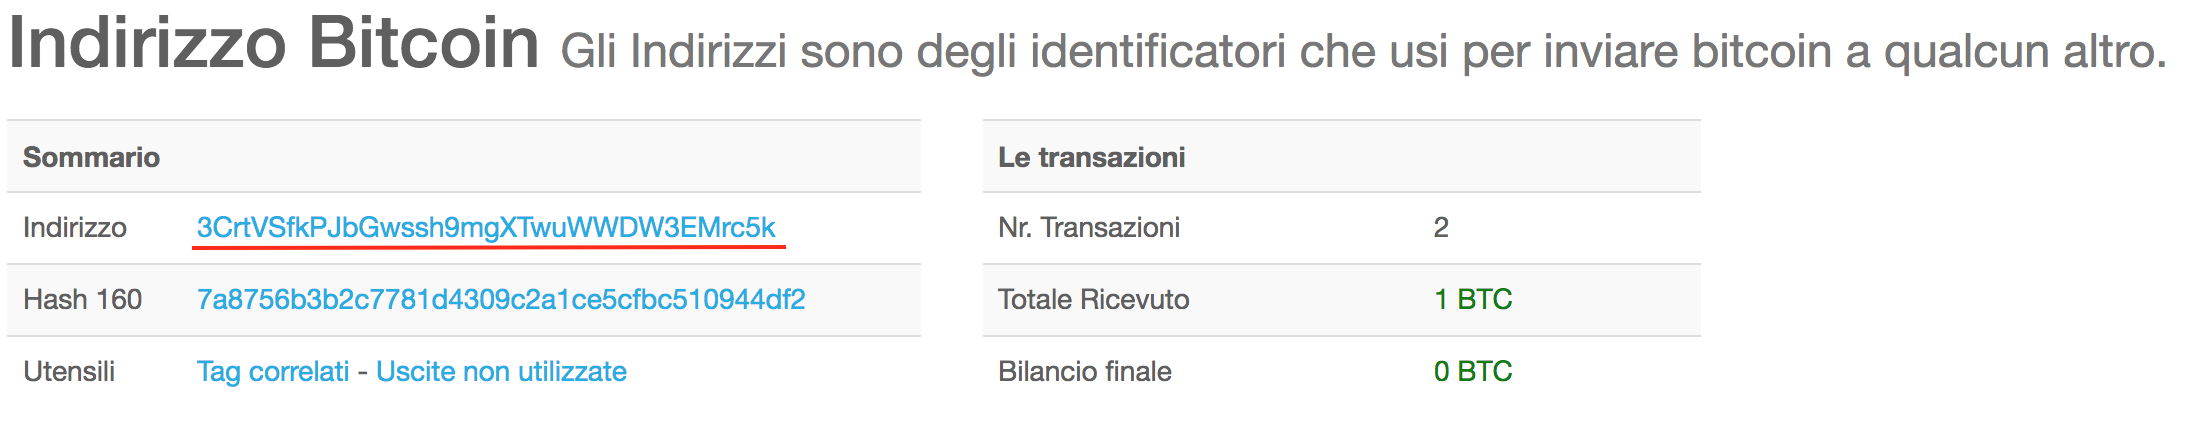
\includegraphics[width=\textwidth]{figure/realtxinput}
		\caption{Input}
		\label{fig:realtxinput}
	\end{subfigure}
	\\
	 %add desired spacing between images, e. g. ~, \quad, \qquad, \hfill etc. 
	%(or a blank line to force the subfigure onto a new line)
	\begin{subfigure}[b]{0.8 \textwidth}
		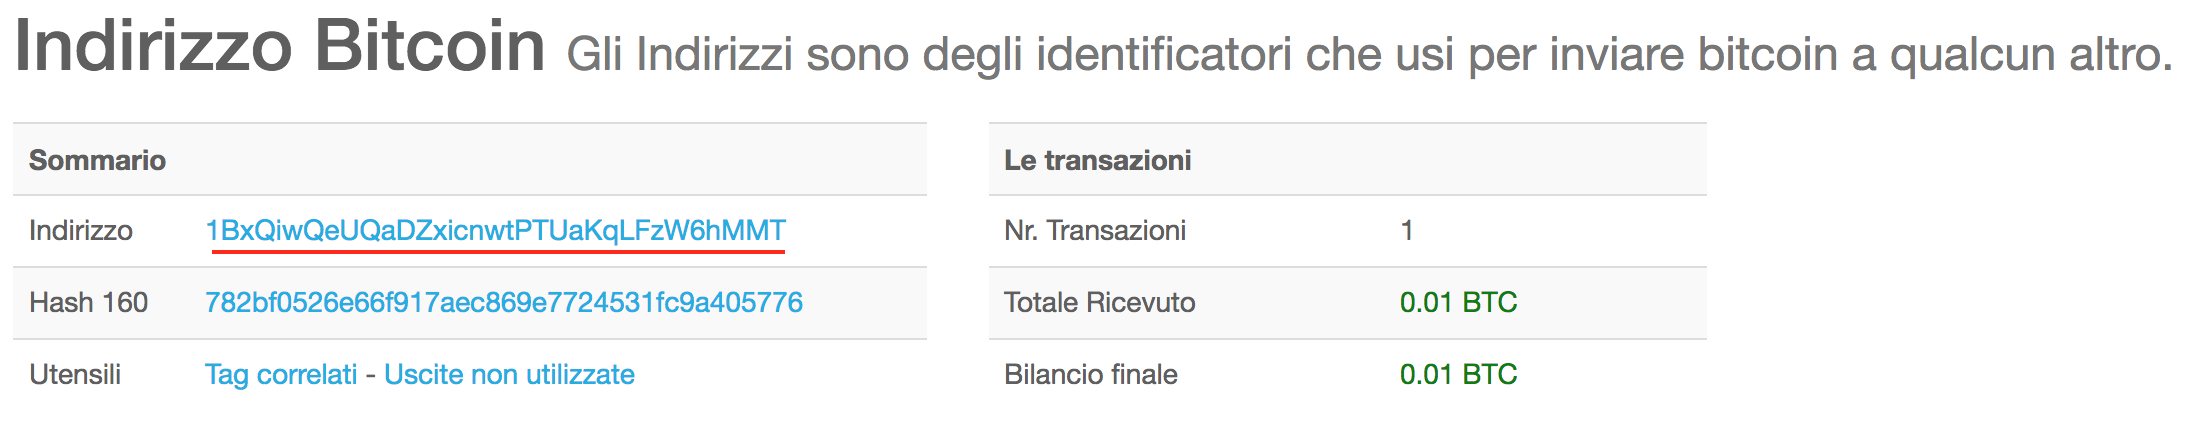
\includegraphics[width=\textwidth]{figure/realtxoutput1}
		\caption{Output 1}
		\label{fig:realtxoutput1}
	\end{subfigure}
	\\
	 %add desired spacing between images, e. g. ~, \quad, \qquad, \hfill etc. 
	%(or a blank line to force the subfigure onto a new line)
	\begin{subfigure}[b]{0.8 \textwidth}
		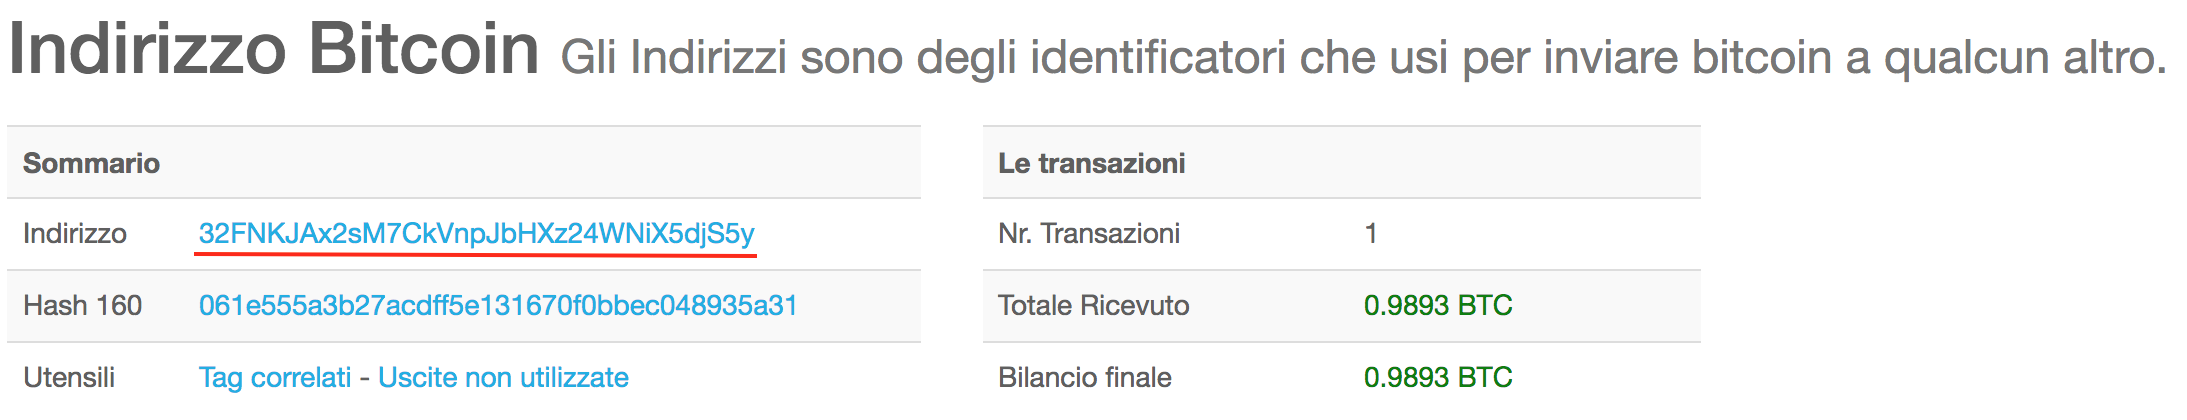
\includegraphics[width=\textwidth]{figure/realtxoutput2}
		\caption{Output 2}
		\label{fig:realtxoutput2}
	\end{subfigure}
	\caption{\textit{Dettagli degli input/output}}\label{fig:realtxdetails}
\end{figure}

Le tre figure soprastanti, rappresentano i dettagli che si possono estrapolare dal sito, riguardo gli indirizzi che intervengono nella transazione. 

Per ogni indirizzo viene indicato il suo identificatore (nel caso di \ref{fig:realtxinput} l'indirizzo è \\ $3CrtVSfkPJbGwssh9mgXTwuWWDW3EMrc5k$) e il suo Hash 160. L'indirizzo stesso è un codice hash, ma non va confuso con il campo \textit{Hash 160}. Quest'ultimo, invece, rappresenta l'hash della chiave pubblica. Più nello specifico, quindi, viene indicato non solo il nome dell'indirizzo, ma anche la chiave pubblica di tale indirizzo, trasformata tramite la funzione hash di crittografia \textit{sha256}.

Il sito \textit{Blockchain.info} mostra, per ogni indirizzo, anche delle statistiche sulle transazioni in cui è stato coinvolto. Infatti, sotto il campo "transazioni" si può osservare che \textit{Nr. transazioni} indica in quante transazioni è implicato tale indirizzo, il campo \textit{Totale Ricevuto} rappresenta il totale di denaro ricevuto e il campo \textit{Bilancio Finale} dovrebbe corrispondere a quanto denaro è rimasto "non speso" ovvero corrisponde ad un UTXO.

Inoltre, ogni volta che si visualizzano tali dettagli, a lato vengono visualizzati anche i corrispondenti QR code, che servono per richiedere ed effettuare i pagamenti.\\

L'anonimia delle transazioni e degli indirizzi bitcoin, viene così sottolineata, in modo tale da mostrare che il sistema bitcoin e la blockchain sono stati pensati per rendere gli scambi di denaro sicuri, veloci, ma anche pubblici, in modo da dare possibilità a chiunque di effettuare una transazione senza utilizzare i propri dati personali. Tutto ciò, visto dal lato generale del sistema complessivo. Prendendo ovviamente in considerazione un esempio in cui, due amici si scambiano denaro in una transazione (come nell'esempio di Alice che compra il caffè al bar di Bob), intuitivamente Alice saprà che tale indirizzo appartiene a Bob e solo a lui, perché potrà verificarlo fisicamente. Perciò, nel più comune caso d'uso di due persone che si conoscono, che si scambiano bitcoin, l'anonimia delle transazioni non viene resa nella misura in cui si vuole far sapere il proprio indirizzo alla persona con cui si sta scambiando denaro. Per esempio, dopo che Alice e Bob hanno fatto la loro transazione, si pensi all'intervento di una persona esterna, Charlie, che non conosce nè Alice nè Bob di persona. Charlie vuole conoscere chi sono i proprietari degli indirizzi della transazione fatta da Alice a Bob, ma non essendoci una corrispondenza diretta tra l'utente fisico e l'indirizzo bitcoin, Charlie non potrà mai scoprire di chi sono tali indirizzi. L'unico caso in cui Charlie li possa scoprire è quello in cui Bob o Alice glieli riveli spontaneamente.

Perciò grazie a questa caratteristica che distingue le transazioni bitcoin da tutte le forme di scambio di denaro fisico, si è portati ad immaginare un altro possibile scenario che verrà trattato nel paragrafo successivo.

\section{Bitcoin Mixing}

Grazie all'anonimia che contraddistingue gli utenti che intervengono nelle transazioni di bitcoin, è possibile pensare che questa caratteristica faciliti lo scambio di denaro all'interno della rete bitcoin. Il rovescio della medaglia però, viene rappresentato da tutti gli utenti che utilizzano la rete per operazioni illecite.

L'anonimia in questione, permette anche allo stesso utente di possedere due o più indirizzi bitcoin diversi. Gli utenti, possedendo ad esempio due indirizzi diversi, vorranno effettuare un certo spostamento di denaro da un indirizzo all'altro. Supponendo che un utente voglia trasmettere una grande quantità di denaro da un indirizzo ad un altro e rendere le transazioni ancora più anonime, egli si rivolge ad un servizio di \textbf{Bitcoin Mixing}.

Il mixing di bitcoin è realmente il riciclaggio di denaro, fatto però attraverso i bitcoin. Il riciclaggio di denaro è quell'operazione che permette di ottenere dei soldi "puliti" a partire da soldi ottenuti in modo illegale, detti "sporchi". Questo processo viene fatto da chi svolge delle attività illegali. Tutto ciò può essere fatto solamente in modo anonimo, proprio per eludere le forze dell'ordine. L'anonimia necessaria viene sfruttata anche attraverso la rete Bitcoin, proprio a causa delle sue caratteristiche. Infatti, nel caso in cui si voglia effettuare un bitcoin mixing ci si deve rivolgere a dei software chiamati Mixer.

\subsection{I Mixer: cosa sono?}

Il software che offre tale servizio è chiamato \textbf{mixer} (letteralmente "miscelatore"). Un mixer svolge quindi l'attività di riciclaggio di bitcoin. Infatti, prendendo in input una certa quantità di bitcoin "sporchi", li "miscela", ovvero crea delle catene di transazioni fittizie con lo scopo di restituire tali soldi "puliti" al mittente (oppure ad un certo indirizzo indicato come output). Il processo viene mostrato nella \textit{figura \ref{fig:mixingschema}}.

\begin{figure}[htbp]
	\centering
	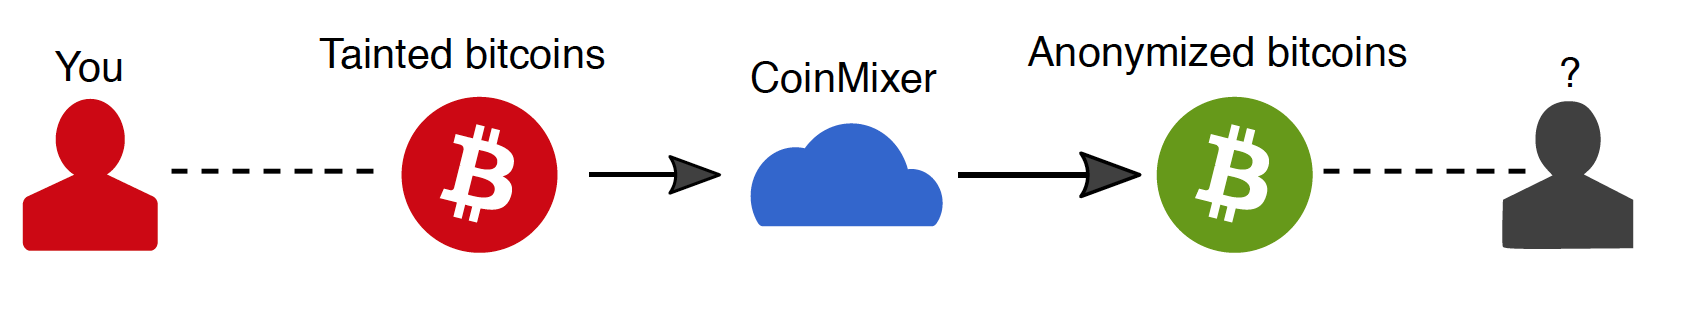
\includegraphics[width = \linewidth]{figure/mixingschema}
	\caption{\textit{Il mixing di bitcoin }\cite{coinmixer}}\label{fig:mixingschema}
\end{figure}

Inizialmente, l'utente intenzionato a usufruire di questo servizio, mette a disposizione del mixer, il denaro che vuole pulire. All'interno di un'interfaccia utente, egli inserisce il proprio indirizzo, l'importo dei bitcoin da riciclare e l'indirizzo di destinazione. Inoltre viene inserito anche un parametro numerico che sta a indicare il numero di ore di ritardo che si può tollerare per ricevere i bitcoin puliti. Ad esempio, se si inserisce 2, il ritardo con cui si riceveranno i soldi sarà pari a 2 ore. Tale parametro rappresenta quindi il tempo necessario affinché il mixer riesca a riciclare i soldi. Più il ritardo è maggiore, maggiormente i bitcoin saranno mixati e resi anonimi, più è vicino a zero, più le transazioni del mixer saranno più facilmente presenti all'interno dello stesso blocco della blockchain.
Esistono dei siti di mixing in cui, nel caso di una grossa quantità di denaro, il ritardo da specificare rappresenta l'intervallo di tempo con cui si vuole riceve ogni fetta dell'intero importo. In questo modo, ogni intervallo di tempo, si riceverà una parte dei soldi riciclati. Così facendo si eluderà maggiormente qualsiasi tentativo di controllo sulle transazioni e sull'automatismo di tali processi.

Il processo che compie un mixer per riciclare i bitcoin, è quello di creare tante transazioni collegate tra loro in una chain, automaticamente, ovvero seguendo un certo algoritmo. Esso prende in input la cifra da riciclare, e distribuisce il denaro tra gli utenti che fanno parte della rete di "riciclatori" del mixer. Successivamente crea ulteriori transazioni da tali utenti verso l'indirizzo indicato come output. E' possibile che il servizio che svolge il riciclaggio abbia un pool di indirizzi dove temporaneamente salva gli importi e, quando richiesto, crei solamente le transazioni di output verso il destinatario. In questo modo non sarà mai possibile collegare il mittente con l'indirizzo di output. 

Questo è proprio l'obiettivo dei siti di mixing, ovvero rendere il denaro più anonimo attraverso transazioni che sembrano "normali", mantenendo l'anonimato e sfruttando la struttura della rete e gli utenti connessi. Il termine "mixing" non assume una accezione negativa nel caso in cui si abbia lo scopo di rendere maggiormente anonime le proprie transazioni. Tuttavia, tale termine potrebbe significare che i bitcoin vengono riciclati esattamente come avviene il riciclaggio del denaro sporco nel mondo reale, creando transazioni irrintracciabili e caratterizzate da una forte anonimia.
\subsection{Mixing nel dettaglio}
L'idea base del mixing è quella di assicurare comunicazioni anonime tra due utenti o indirizzi.

 La \textit{figura \ref{fig:mixingschema}} mostra l'idea di base, la relazione tra Alice e Bob viene nascosta dal servizio di mixing.
\begin{figure}[htbp]
	\centering
	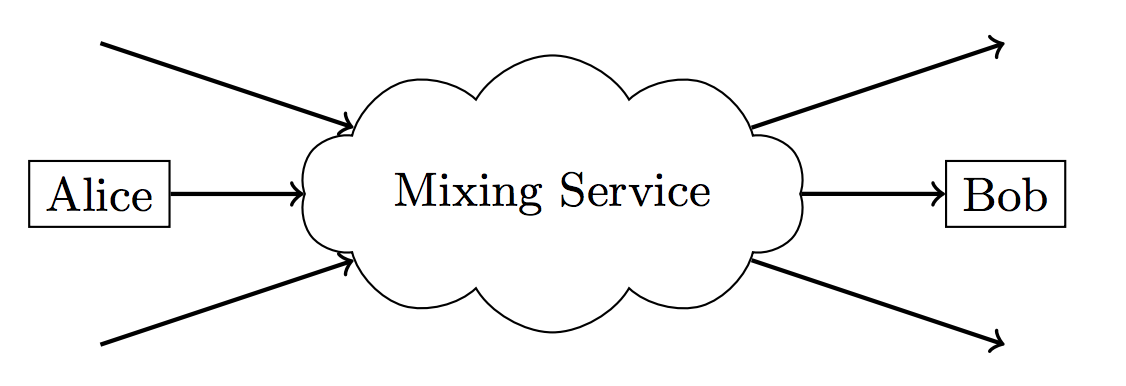
\includegraphics[width = 0.7 \linewidth]{figure/moesermixservice}
	\caption{\textit{Un servizio di mixing, che nasconde la relazione tra Alice e Bob}}\label{moesermixservice}
\end{figure}

Un mixer prende un insieme di input, che sono stati criptati con la chiave pubblica $c_M$ del mixer e contiene un messaggio criptato $c_A(z_0,m)$, un indirizzo A di destinazione, e una stringa random $z_1$ che serve per mantenere la dimensione del messaggio in arrivo uguale a quella del messaggio in uscita.

Ricevute le informazioni, il mixer decripta il messaggio, rimuove la stringa random (equazione \eqref{eq:mixingequation}) ottenendo il messaggio di lunghezza giusta, e lo cripta di nuovo in base all'indirizzo associato a cui deve mandarlo.

\begin{equation}
	\centering
	c_M(z_1,c_A(z_0,m),A) \to c_A(z_0,m),A
	\label{eq:mixingequation}
\end{equation}

Al fine di ridurre il pericolo che un singolo mixer venga attaccato da un hacker, che potrebbe conoscere la relazione tra gli input e gli output, molti mixer vengono collegati insieme, creando un mixing a cascata. L'utente successivamente dovrà decriptare il messaggio con tutte le chiavi pubbliche dei vari mixer, e ciò assicura che ogni mixer ha ricevuto solamente il messaggio criptato e il successivo indirizzo di destinazione.\cite{moser2013anonymity}

\subsection{Tor}

\begin{wrapfigure}{l}{0.2 \textwidth}
	\vspace{-20pt}
	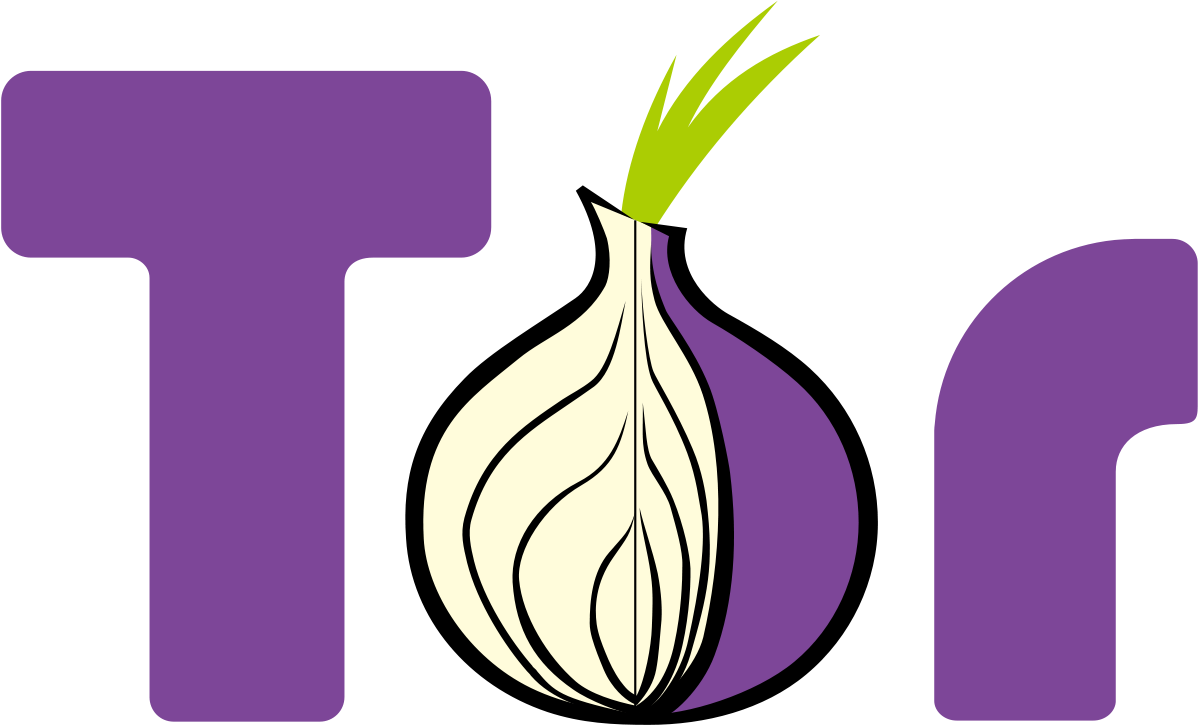
\includegraphics[width=0.15\textwidth]{figure/torlogo}
\end{wrapfigure}
A causa di questo processo, tutto ciò non è praticabile all'interno di una rete internet standard. Infatti, per usufruire dei software di mixing occorre essere connessi ad internet tramite il browser Tor.

In informatica \textbf{Tor}(acronimo di The Onion Router) è un sistema di comunicazione anonima per Internet basato sul protocollo di rete di \textit{onion routing}. Tramite l'utilizzo di Tor è molto più difficile tracciare l'attività Internet dell'utente; difatti l'uso di Tor è finalizzato a proteggere la privacy degli utenti, la loro libertà e la possibilità di condurre delle comunicazioni confidenziali senza che vengano monitorate. \textit{Onion routing} è una tecnica per rendere anonime le comunicazioni all'interno della rete. In una rete onion (letteralmente "cipolla"), i messaggi sono incapsulati in "strati" di crittografia che vengono paragonati agli strati di una cipolla. \cite{wiki:tor}

Il mixing dei bitcoin e lo scambio illecito di denaro, può essere intercettato in una rete internet standard. Tor, quindi è una rete secondaria che permette lo scambio di transazioni di denaro (e altro), che su un normale browser non sarebbe possibile. Infatti, essendo propriamente una rete nascosta è difficile intercettarne i pacchetti e capire quali scambi vengano fatti. Questo perché, proprio il protocollo con cui è stata pensata non permette che si spoofi la comunicazione tra due utenti. La caratteristica principale si può dedurre dal nome della tecnologia, the onion router. Letteralmente "onion" significa cipolla, e sta ad indicare la stratificazione che accomuna tali pacchetti con il tubero puzzolente. 
I pacchetti della rete tor sono letteralmente stratificati, ossia ogni volta che viene aggiunto uno strato, si applica una funzione di crittografia. Una terza persona che riesce a sniffare un pacchetto di questo tipo, non riuscirà ad aprirlo, anche conoscendo le chiavi del ricevente e del destinatario.

Tali pacchetti sono adatti alla topologia della rete tor, poichè la rete è pensata per rendere anonime le comunicazioni. Tale anonimia è resa dal fatto che i pacchetti non seguono un algoritmo di instradamento, ma letteralmente "rimbalzano" da un router ad un altro, arrivando infine a destinazione. Proprio per tale caratteristica, la connessione tor appare lenta, poichè la trasmissione del pacchetto impiega più tempo ad arrivare a destinazione, più di un normale pacchetto.

I messaggi, quando vengono trasmessi, è come se seguissero la strada più lunga attraverso la rete, passando anche più volte per gli stessi router. La stratificazione infatti viene realizzata ad ogni singolo passaggio di un pacchetto attraverso un router. Così facendo, il successivo router destinatario, toglierà man mano uno strato di crittografia.
